\RequirePackage{shellesc}
\documentclass[a4paper]{article}
\usepackage[document]{ragged2e}
\usepackage{fontspec}
\usepackage{geometry}
\usepackage{titlesec}
\usepackage{graphicx}
\usepackage{float}
\usepackage{minted}
\usepackage{enumitem}
\usepackage[Export]{adjustbox} % Used to constrain images to a maximum size
\usepackage[font=large]{caption}
\geometry{left=2cm}
\geometry{right=2cm}
\geometry{top=2cm}
\geometry{bottom=2cm}
\setmainfont{Liberation Serif}
\setmonofont[Scale=0.7]{Hack}
\titlelabel{\thetitle. }
\renewcommand{\tablename}{Таблица}
\renewcommand{\figurename}{Рисунок}
\counterwithin{table}{section}
\counterwithin{figure}{section}
\captionsetup{justification=raggedright,singlelinecheck=false}
\renewcommand\large{\fontsize{14}{16}\selectfont}
\renewcommand{\theFancyVerbLine}{\textbf{\arabic{FancyVerbLine}}}
\sloppy

\setminted{
  linenos,
  breaklines,
  breakanywhere,
  breaksymbolleft=,
  fontsize=\fontsize{12}{12}\selectfont,
  numbersep=5pt,
}
\usemintedstyle{emacs}

\graphicspath{ {./pics/} }

\begin{document}
  \fontsize{14}{16}\selectfont

  \begin{titlepage}
    \begin{minipage}{0.2\textwidth}
      
\includegraphics[scale=0.4]{logo}
    \end{minipage}
    \begin{minipage}{0.7\textwidth}\centering
      \fontsize{10}{12}\selectfont
      \textbf{
        Федеральное государственное бюджетное образовательное учреждение \\
        высшего профессионального образования \\
        «Московский государственный технический университет имени Н.Э. Баумана» \\
        (МГТУ им. Н.Э. Баумана)
      }
    \end{minipage}

    \vspace{5cm}
    \centering
    \fontsize{16}{20}\textbf{
      Лабораторная работа №4 \\
      по курсу «Методы машинного обучения» \\
    }

    \vspace{5cm}
    \begin{flushright}
    Выполнил \\
    студент группы ИУ5-22М \\
    XXXX \\
    \end{flushright}
    \vspace*{\fill}
    Москва, 2023
  \end{titlepage}

  \justifying
  \setlength{\parindent}{1.25cm}

  \section{Задание}
  \begin{enumerate}[leftmargin=1.25cm]
    \item На основе рассмотренного на лекции примера реализуйте алгоритм Policy Iteration
      для любой среды обучения с подкреплением (кроме рассмотренной на лекции среды Toy Text / Frozen Lake)
      из библиотеки Gym (или аналогичной библиотеки).
  \end{enumerate}

  \section{Текст программы}
  \inputminted{python}{4.py}

  \section{Экранные формы с примерами выполнения программы}
  \begin{minted}{text}
$ ./4.py
1000 шагов.
Стратегия:
array([[0. , 0. , 0. , 0. , 1. , 0. ],
       [0. , 0. , 0. , 0. , 1. , 0. ],
       [0. , 0. , 0. , 0. , 1. , 0. ],
       ...,
       [0. , 1. , 0. , 0. , 0. , 0. ],
       [0. , 0.5, 0. , 0.5, 0. , 0. ],
       [0. , 0. , 0. , 1. , 0. , 0. ]])
  \end{minted}
  \begin{figure}[H]
    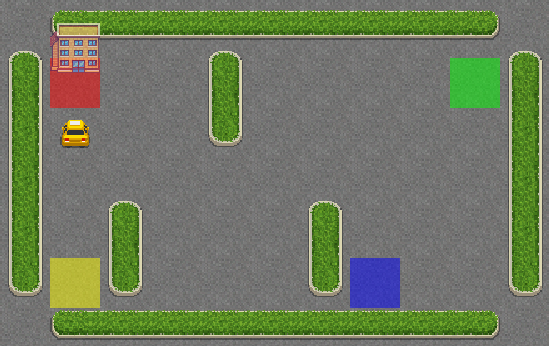
\includegraphics[scale=0.5]{41}
  \end{figure}
\end{document}
